\section{Iteración II}
\subsection{Resumen}
En esta iteración se modeló un mueble y se implementó para visualizarse en la aplicación.
\subsection{Desarrollo}
Ya entendido el funcionamiento de ARcore y como agregar nuevos modelos, en esta iteración se realizó el modelado de un objeto de mayor complejidad: una mesa metálica con algunos detalles de acabado. Al igual que en la iteración pasada se obtuvieron dos tipos de archivos y se renderizaron para mostrarse en la aplicación. El resultado de esta iteración es el equivalente al entregable de TT I que propusimos en el protocolo, en donde planeamos que al final de la iteración IV ibamos a entregar una aplicación que a través de realidad aumentada pudiera mostrar un simple mueble sin cambios de color o textura.
En la figura 4.28 se puede observar el nuevo modelo implementado.
\begin{figure}[H]
	\centering
	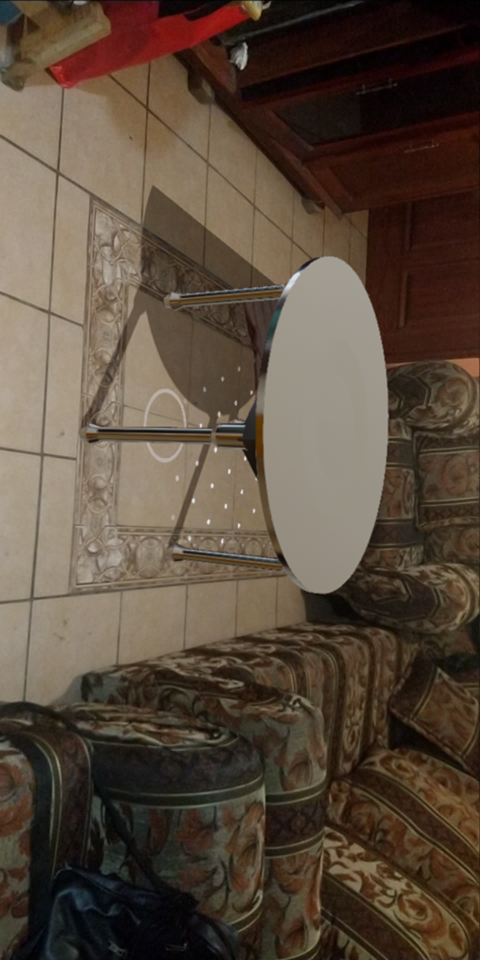
\includegraphics[width=8cm,height=14cm,angle=90]{imagenes/iteraciones/AR3.png}
	\caption{Mueble modelado en 3D}
	\label{fig:analogo}
\end{figure} 
\clearpage